\subsubsection{Modèle basé sur les règles expertes}\label{regles}

%La troisième couche consiste à classer l'instance en deux classes (\textit{alerte} et \textit{non alerte}) selon des règles expertes.  
%Comme il n'est pas possible de compter en permanence sur la participation du professionnel pour étiquer les messages et calculer l'estimation des pertes, 
Nous avons également implémenté des règles expertes fournies par l'association \textit{OADI} pour la levée de l'alerte et nous avons exploré les scénarios suivants. Une alerte est levée si il y a : 
1) un message avec un risque  de niveau 4 dans les $N$ derniers messages;
2)  une augmentation du niveau de risque entre 2 temps consécutifs;
3)  une augmentation du niveau de risque avec un écart de au moins 2 niveaux sur une fenêtre de $N$ messages; Nous ferons varier $N$ pour évaluer les performances pour détecter des changements abrupts ou lents;
4)  des oscillations du niveau de risque.

On obtient alors les règles suivantes : Soit $M$ l'ensemble des $N$ derniers messages d'un utilisateur où $M_1$ correspond au message le plus ancien et $M_N$ au plus récent. On notera $R_i$ le niveau de risque du message $i$.

% * <jeromeaze@gmail.com> 2015-09-21T10:03:18.541Z:
%
%  Dans le contexte, je ne comprend pas 
%
\begin{itemize}
\item  $\exists i, 0\leq i \leq N | R_i = 4$
\item  $\exists i, 0\leq i \leq N-1 | R_i < R_{i+1}$
\item  $\exists i, 0\leq i \leq N-1 | R_i < (R_{i+1}-1)$
\item  $\exists i \exists j, 0\leq i \leq N-1, 0\leq j \leq N-1 | R_i < R_{i+1}, R_j > (R_{j+1})$
\end{itemize}

\begin{figure}[!h]
   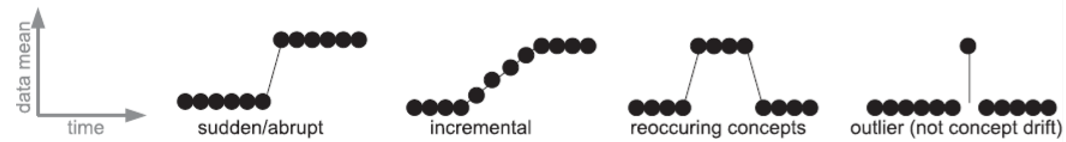
\includegraphics[width=.95\textwidth]{imgs/types_concept_drift.png}
	\caption{\label{formes_cd} Les différentes formes de \emph{concept drift} (adaptés de \cite{Gama2014})}
\end{figure}

Le schéma \ref{formes_cd} représente les différentes formes de changement que nous souhaitons capturer via les règles expertes : 
1) Le changement \emph{immédiat} correspond à un individu qui parle du jour au lendemain de méthode de suicide;
2) Le changement \emph{incrémental} correspond au cas où l'individu parle de plus en plus de son mal être;
3) Le changement \emph{récurrent} est un utilisateur qui régulièrement parle de son mal être;
4) Le \emph{bruit} serait un message isolé parlant de suicide.